\chapter{Введение}

%Пример работы в ОС Linux на примере дистрибутива Debian.
Соглашения и обозначения:

\begin{itemize}
	\item \keys{ Esc } -- нажатие клавиши Esc
	\item \cmd{pwd} -- команда консоли (программа)
	\item \cfgfile{/etc/passwd} -- конфигурационный файл или файл с настройками
	\item \cfgpath{/proc/} -- путь к директории с файлами процессов
\end{itemize}

%\section{vi}
%\section{nano}
%\section{базовые команды}
%\section{регулярные выражения}
%\section{командая строка и bash}
%\section{экранные менеджеры screen, tmux}
%\section{философия unix}
%\section{иерархия файлов}

%\begin{figure}
	%\centering
%	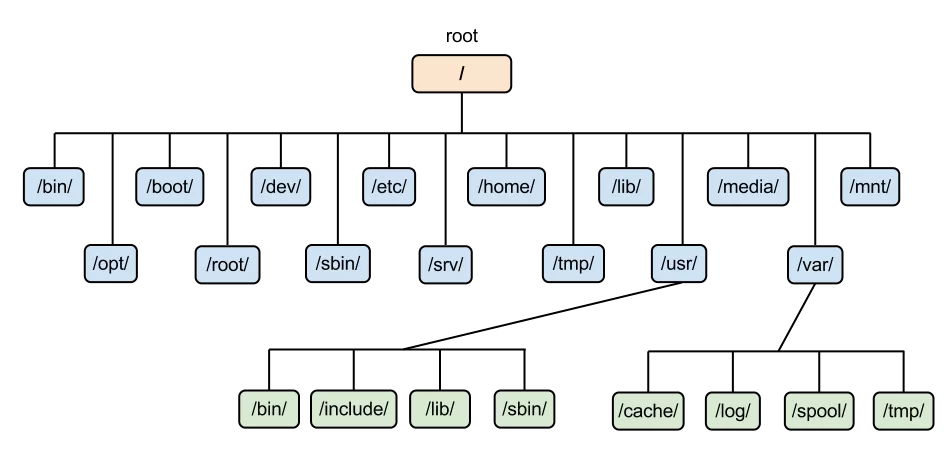
\includegraphics[width=\textwidth]{img/ch1/hfs.png}
%	\caption{Иерархия файловой системы}
%	\label{fig:galaxy}
%\end{figure}

%\keys{Сtrl + Shift + F}

%man -K IPX

%\texttt{man}

%\keys{Сtrl + Shift + F}
